\documentclass{beamer}
\usepackage{graphicx}

\title[Bees?]{``Bees?''\\ A Large Scale, Co-operative Simulation Weighing
                          Altruism and Selfishness}
%\author{A. Simms, R. Thielstrom}
\institute{Swarthmore College}
\date{Adaptive Robotics, Spring 2014}

\usetheme{Luebeck}
\usecolortheme{crane}
\begin{document}

    \begin{frame}
        \titlepage
    \end{frame}

    \begin{frame}
        \tableofcontents
    \end{frame}


    \section{Overview}

    \begin{frame}{Overview}
        \begin{itemize}
            \item Attempting to investigate conditions for selfishness and altruism in a community
                  of neural-net agents.
            \item Can we get co-operation from a large number of independent agents?
            % \item 
        \end{itemize}
    \end{frame}

    \section{Experiment}

    \subsection{Bees?}
    \begin{frame}{The Bee model}
        \begin{itemize}
            \item Many individual ``bees'' in a ``hive''.
            \item Each bee is an individual NEAT agent.
        \end{itemize}
    \end{frame}

    \begin{frame}{A day in the life of a bee}
        Every ``day'' in the simulation:
        \begin{itemize}
            \item Each bee goes out to get ``nectar''
            \item Has the decision to eat the nectar there, or bring it back to the hive
            \item At the hive, the nectar brought back by the bees is shared equally between 
                  the bees that brought back nectar
        \end{itemize}
        With a specified lifetime of days, fitness is determined by the avg nectar a bee accumulates throughout its lifetime.
    \end{frame}

    \subsection{Implementation}
    \begin{frame}{NEAT Implementation}
        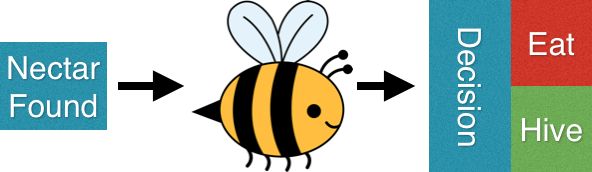
\includegraphics[height=3cm]{bee.png}
        \begin{itemize}
          \item Other varied inputs: last decision, hive nectar, majority decision, last fitness, last guidance decision
    \end{frame}

    \section{Hypothesis}

    \subsection{Hypothesis}
    \begin{frame}{Hypothesis}
            \begin{itemize}
                    \item We predict that the amount of altruism and selfishness demonstrated in 
                          NEAT-trained agents will be most affected by an individual fitness relying
                          on overall group fitness.

            \end{itemize}
    \end{frame}

    
    \subsection{Experimental Ideas}
    \begin{frame}{Most conducive environments to altruism}
        \begin{itemize}
            \item Incentivize altruism with explicitly higher fitness.
            \item Deincentivize selfishness with explicitly lower fitness.

            \item Some way of tying ``sharing'' fitness.
            \begin{itemize}
                \item The ``hive'' has an amount of honey to support the ``queen,'' and this 
                      influences fitness.
                \item Have all of the bees share the fitness of the hive.
                \item Have the health of the hive worked into the fitness function in another way
            \end{itemize}
        \end{itemize}
    \end{frame}



    \section{Experiments}

    \subsection{Basic Experiments}

    \begin{frame}{Basic Experiments}
        \begin{figure}
            
        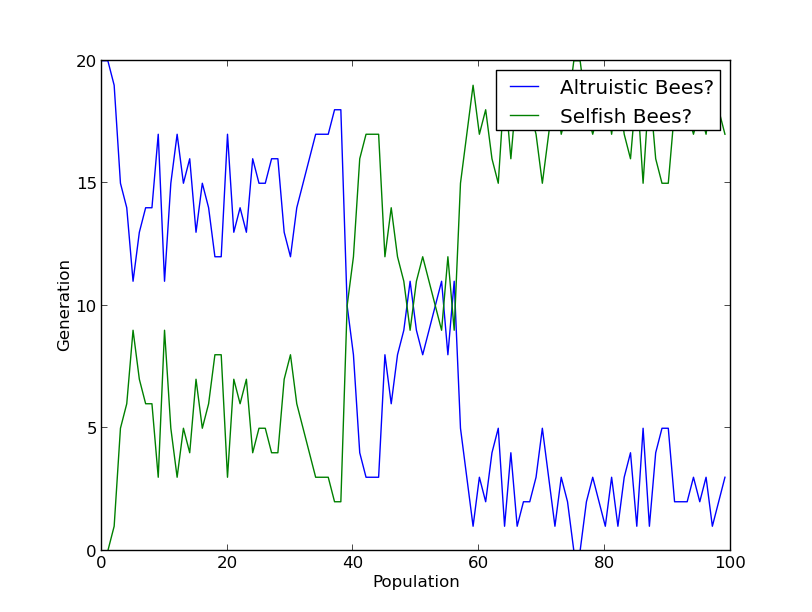
\includegraphics[width=8cm]{s_bees.png}
        \end{figure}

    \end{frame}

    \subsection{Hive-Based Fitness}

    \begin{frame}{Added notion of ``Hive'' fitness}
        \begin{itemize}
            \item The hive has some ``nectar reserves''.
            \item Maintained by taking some nectar from the bees that brought back nectar.
            \item A pentalty is assessed to the fitness of all bees if nectar drops below a certain 
                  level.
        \end{itemize}
    \end{frame}


    \begin{frame}{The Only Difference is Hive Fitness}
        \begin{figure}
            
        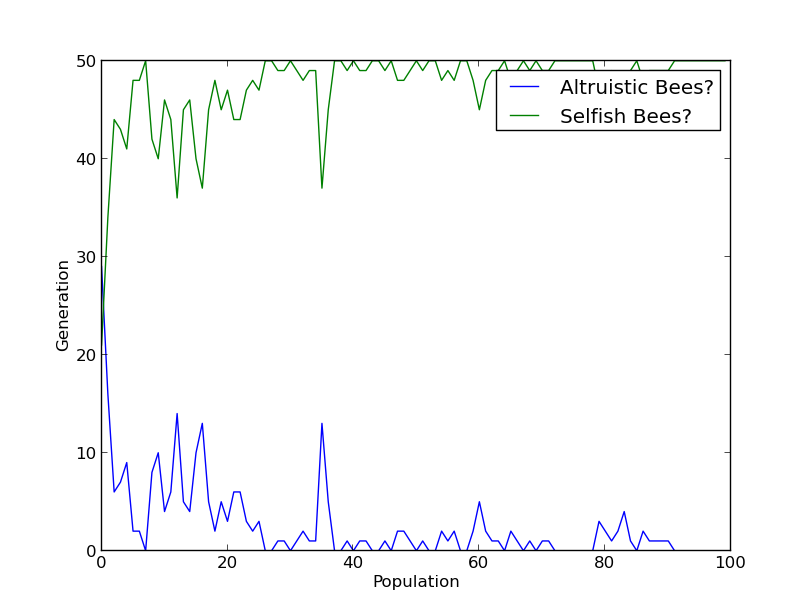
\includegraphics[width=8cm]{hive_influenced_bees.png}
        \end{figure}
    
    \end{frame}

    \begin{frame}{``Nectar Reserves'' Over Time}
        \begin{figure}
        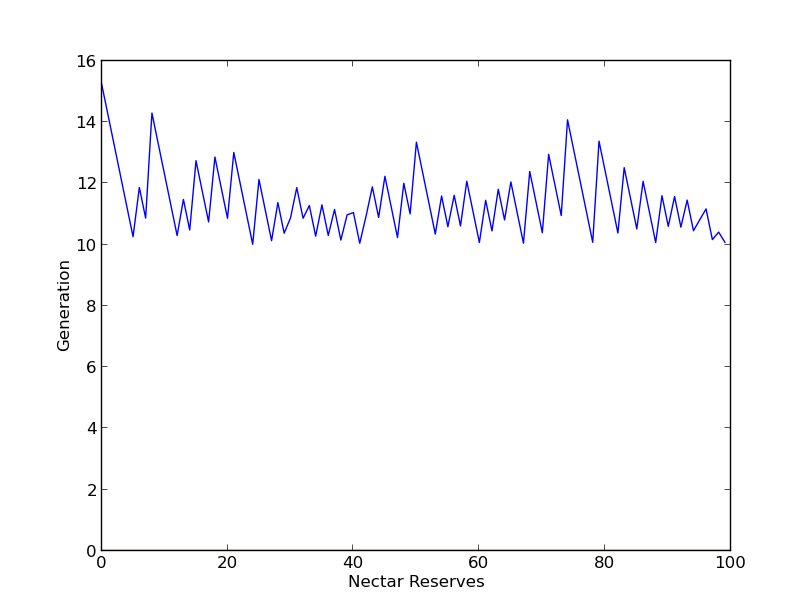
\includegraphics[width=8cm]{hive_influenced_bees_nectar.png}
        \end{figure}
    \end{frame}

    \section{Data Analysis}
    \begin{frame}{Data Analysis}
        \begin{itemize}
          \item Hive fitness not only deducts fitness for hive-endangering bees but also reduces the possible benefits of altruism
          \item Selfishness will initially always be the ``better'' option


    \section{Q and A}
    \begin{frame}{Questions?}
        \titlepage
    \end{frame}

\end{document}
